\chapter{System Description}
\label{ch:sysDescription}

The subject of this study's modeling effort is the Model for Aeroelastic Response to Gust Excitation (MARGE). MARGE is a flexible half-span wing-body-tail wind tunnel model which is capable of rigid-body rotation in the pitch axis. It was designed to allow rapid and accessible testing of gust alleviation control laws. Thus, it is of a simple and affordable construction. Details of the original design and construction of MARGE can be found in \cite{Quenzer2019}.

The structure of MARGE consists of flexible beams encapsulated by lightweight aerodynamic shells. The wing and tail spars are made of aluminum while the fuselage is made of steel. The aerodynamic shells are made of polylactic acid (PLA) and form a symmetrical NACA 0012 airfoil. There is a brass mass fixed at the wing tip to bring the structure's natural frequencies to the designed magnitude. The wing is joined to the fuselage at its root and the entire assembly rotates about a shaft which is suspended from the hanging sub-assembly by bearings. A diagram of the structural configuration of MARGE is shown in Fig. \ref{fig:structureConfig}.
\begin{figure}[h]
    \centering
    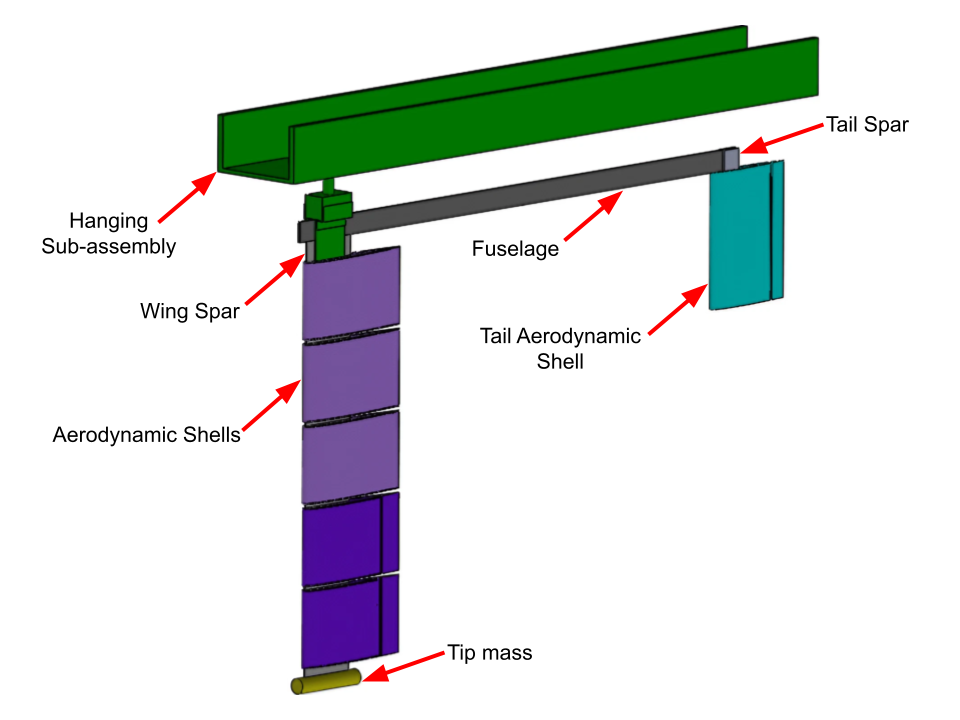
\includegraphics[width=0.75\textwidth]{structConfig.png}
    \caption{MARGE structural configuration}
    \label{fig:structureConfig}
\end{figure}

MARGE has three actuators: two servo-actuated control surfaces on the wing and one servo-actuated elevator on the tail. There are also two servo-activated gust vanes installed upstream of the test section in the 3x3 low-speed wind tunnel. The gust vanes move in unison to generate discrete or continuous gusts and are controlled as a single actuator.

MARGE has five sensors. There are two unidirectional accelerometers at the wingtip, one ahead of the wing spar and one aft of the wing spar. There is another unidirectional accelerometer at the tip of the tail. (All three accelerometers are aligned normal to the lifting surfaces.) There is a strain gauge at the wing root. Finally, there is a hall effect sensor inside the hanging sub-assembly by the model's rotating shaft. There is a magnet fixed to the shaft which allows the hall effect sensor to measure the rotation of the shaft. A diagram of the sensing and actuation configuration of MARGE is shown in Fig. \ref{fig:sensorConfig}.

Note that the sensor configuration is modified from the original design specified in \cite{Quenzer2019}. The original design featured potentiometers on the control surfaces and a strain gauge on the fuselage. It also lacked the accelerometer on the tail. The potentiometers and the fuselage strain gauge have since been removed because they were found to be unnecessary. The accelerometer on the tail has since been added with the intent of capturing fuselage and tail flexible motions.
\begin{figure}[h]
    \centering
    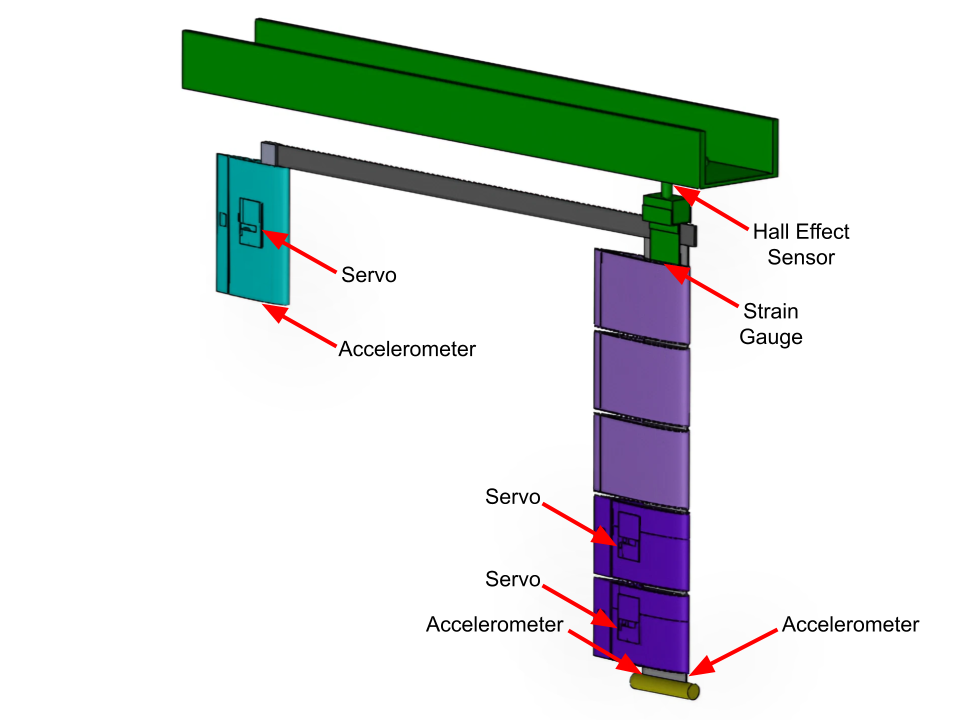
\includegraphics[width=0.75\textwidth]{sensorConfig.png}
    \caption{MARGE sensing and actuation configuration}
    \label{fig:sensorConfig}
\end{figure}

MARGE is designed to fit into the University of Washington's 3x3 low-speed wind tunnel. The 3x3 low-speed wind tunnel is an open-loop wind tunnel capable of speeds up to 60 m/s. The wind tunnel has flow straighteners, a 9:1 contraction, gust vanes, and a 3 ft. by 3 ft. by 8 ft. test section. Further details about the 3x3 low-speed wind tunnel can be found in \cite{3x3site}. When installed, MARGE hangs vertically from the ceiling of the test section. A diagram indicating the key features of the 3x3 low-speed wind tunnel is shown in Fig. \ref{fig:3x3}.
\begin{figure}[h]
    \centering
    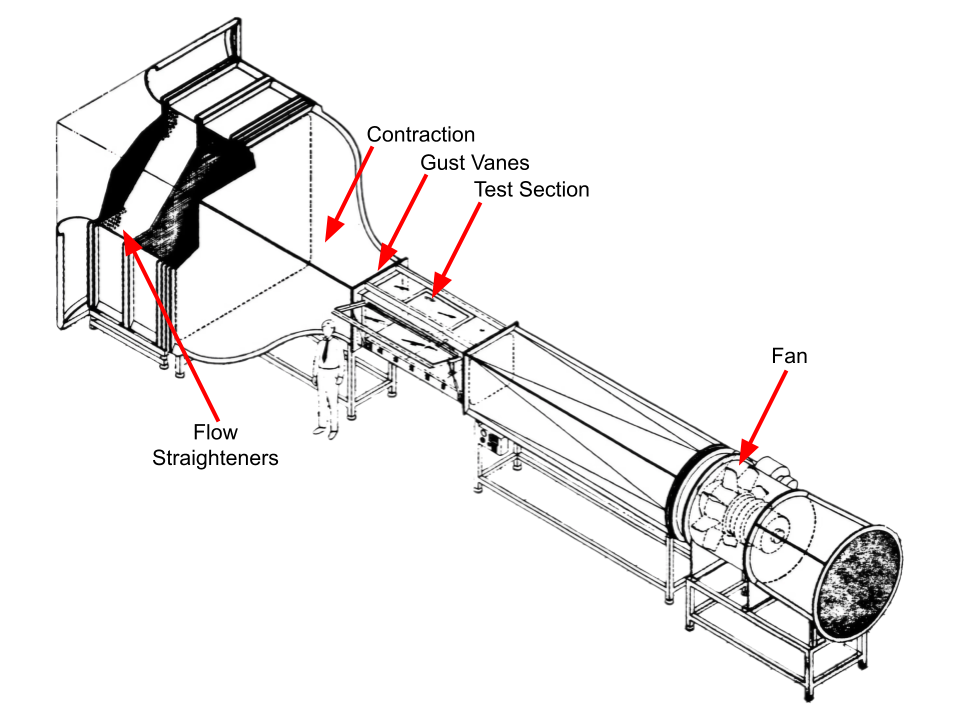
\includegraphics[width=\textwidth]{windTunnelIsoDiagram.png}
    \caption{Univeristy of Washington 3x3 low-speed wind tunnel}
    \label{fig:3x3}
\end{figure}

The physical interface to MARGE's acutation and sensing is a National Instruments DAQ coupled with a National Instruments terminal block. The exceptions to this are the gust vanes, which are controlled through HTTP on the local network. Data is transmitted and received to and from these interfaces through Simulink Real-Time.